\subsection{Worksheet - Review of Weeks 1-4}
\begin{p}
Which of these problems must be solved using the calculus of variations?
\newline 1. Find the period of small oscillations for a particle sliding (without friction) on the inside of a sphere.
\newline 2. Find the surface with fixed area that encloses the maximum volume.
\newline 3. Find the path between two points that minimizes the time for a particle to slide (without friction) between the points.
\newline 4. Find the path of a projectile (with no air resistance) that leads to the maximum range.
\end{p}
\begin{s}
Exactly two. For 1, we looked at the equations of motion and Taylor expanded around the minimum for small $\phi$. So, we aren't looking for the path that minimizes some functional in this case, hence its not particularly a variational problem. For 2, we have an optimization problem; we are trying to extremize/maximize a volume. We can write an expression for the surface area, and add in a constraint (e.g. we could use Lagrange multipliers for example). We could optimize this with the Calculus of variations. 3 is the brachistochrone problem, obviously yes. 4 does not require varations; this is just a question of initial conditions of the trajectory.
\end{s}

\begin{p}
A calculus of variations problem requires minimizing
$$
J[y(x)]=\int_{x_{1}}^{x_{2}} f\left[y(x) ; y^{\prime}(x) ; x\right] d x
$$
When we solve Euler's equation
$$
\frac{\partial f}{\partial y}-\frac{d}{d x} \frac{\partial f}{\partial y^{\prime}}=0
$$
what do we learn?
\end{p}
\begin{s}
We learn of the path $y(x)$ that minimizes $J[y(x)]$; the EL equation gives a differential equation for the path $y(x)$ which minimizes $J[y(x)]$.
\end{s}

\begin{p}
What is the Lagrangian of a particle of mass $m$ attached to a spring with spring constant $k$?
\end{p}
\begin{s}
$\LL = T - U = \frac{1}{2}m\dot{x}^2 - \frac{1}{2}kx^2$ (the kinetic energy term minus the potential energy term).
\end{s}

\begin{p}
What is the Lagrangian of a pendulum of mass $m$, length $l$? Assume the potential energy is zero when $\theta$ is zero.
\end{p}
\begin{s}
$\LL(\theta, \dot{\theta}, t) = \frac{1}{2}ml^2\dot{\theta}^2 - mgl(1-\cos\theta)$
\end{s}

\begin{p}
For which of these systems could you use Lagrange's equations of motion?
\newline 1. A double pendulum: a pendulum (mass $\mathrm{m}$, length 1 ) has a second pendulum (mass $\mathrm{m}$, length l) connected to its bob.
\newline 2. A projectile moves in two dimensions with gravity and air resistance.
\newline 3. A bead slides without friction on a circular, rotating wire.
\end{p}
\begin{s}
Everything but 2 works; with 2, we have friction/a non-conservative force and hence the Lagrange equations no longer apply (though we can add in a correction to account for this).
\end{s}

\begin{p}
A particle moves in one dimension with Lagrangian $\LL = T - U$. Suppose we shift the potential energy $U$ by a constant $C$. What changes?
\end{p}
\begin{s}
The value of $S$ changes ($S$ depends on the Lagrangian) but the physical path $x(t)$ taken by the particle remains invariant (that is, the path that gives $\delta S = 0$); one way of seeing this is the equations of motion are given by derivatives of the Lagrangian, which would remove the effects of any constants.
\end{s}

\begin{p}
A bead of mass $m$ slides on a circular wire of radius $R$, which rotates about a vertical axis with angular velocity $\Omega$. The equation of motion of the bead is \[\ddot{\theta} + \frac{g}{R}\sin\theta - \Omega^2\sin\theta\cos\theta = 0\]
What are the equilibrium values of $\theta$?
\end{p}
\begin{s}
$\theta = 0,\pi$ and $\theta = \pm\arccos(\frac{g}{R\Omega^2})$.
\end{s}

\begin{p}
The equation of motion for small motions about the equilibrium $\theta = \arccos(\frac{g}{R\Omega^2})$ above is given by:
\[\ddot{\theta} +\Omega^2\sin^\theta_0\theta = 0\]
What is the oscillation frequency of the bead?
\end{p}
\begin{s}
$\omega = \Omega\sin\theta_0$
\end{s}

\begin{p}
Which of these systems are holonomic? E.g. which of these systems have a constraint that can be written as $f(q_1, \ldots, q_n, t) = 0$?
\newline 1. The double pendulum, but with the lower mass attached by a spring instead of a spring.
\newline 2. The motion of a hockey puck around a frictionless air hockey table
\newline 3. A bead moving frictionless on a circular wire hoop spinning at fixed angular velocity.
\end{p}
\begin{s}
A and C. With C, this is obviously possible (we constrain the radius). With B, the constraint is an inequality (e.g. the normal force is just such that the mass stays at the level of the table), which makes it non-holonomic. With A, we have that the lower mass can move more freely; the system is still holonomic, we just got rid of the constraint on the second mass. Note that if forces are dissipative, then we can also not write constrains as holonomic.
\end{s}

\begin{p}
What is the constraint equation?
\begin{center}
    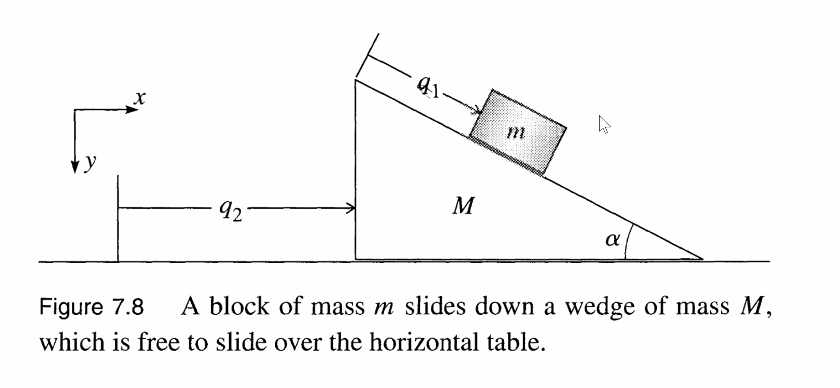
\includegraphics[scale=0.75]{Lecture-13/w13-img1.png}
\end{center}
\end{p}
\begin{s}
$f(x,y) = \frac{y}{x} - \tan(\alpha) = 0$. A typical holonomic constraint.
\end{s}

\begin{p}
A particle of mass $m$ slides on the outside of a cylinder of radius $a$. A good choice of generalized coordinates is $(r, \theta)$. What is the constraint equation?
\end{p}
\begin{s}
$f(r,\theta) = r - a = 0$
\end{s}

\begin{p}
What can you conclude from the fact that $\dpd{\LL}{\dot{x}_i}$ is constant for all $i$?
\end{p}
\begin{s}
Momentum is conserved.
\end{s}

\begin{p}
How can we rewrite:
\[\int_{t_1}^{t_2}p_j\dod{}{t}\delta q_j dt\]
\end{p}
\begin{s}
By integrating by parts, we get:
\[-\int_{t_1}^{t_2}\dot{p}_j\delta q_j dt\]
(the variation vanishes at the boundary, so it is discarded).
\end{s}
